%! Author = gramic
%! Date = 21.04.24

% Preamble
\begin{flushleft}
    \subsection{Maintenance - Patroni}
    \label{subsec:maintenance_patroni}
    Patroni wird von Zalando regelmässig gepflegt.
    Das Projekt hat eine überschaubare Anzahl an Issues, wird aber Regelmässig
    \begin{figure}[H]
        \centering
        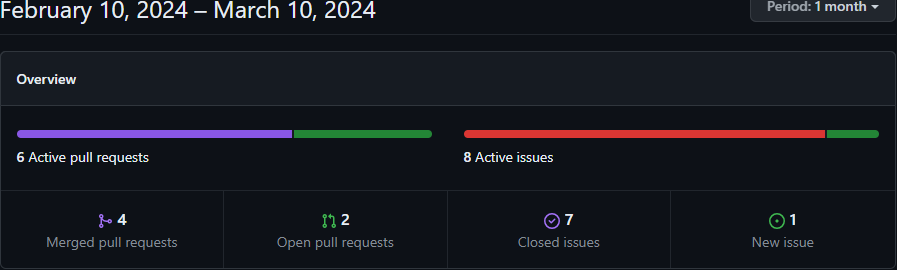
\includegraphics[width=0.75\linewidth]{source/implementation/evaluation/postgresql_ha_solutions/insights/patroni/pulse_zalando_patroni}
        \caption{Patroni - Pulse}
        \label{fig:pulse_zalando_patroni}
    \end{figure}

    Code wird Regelmässig hinzugefügt und entfernt:
    \begin{figure}[H]
        \centering
        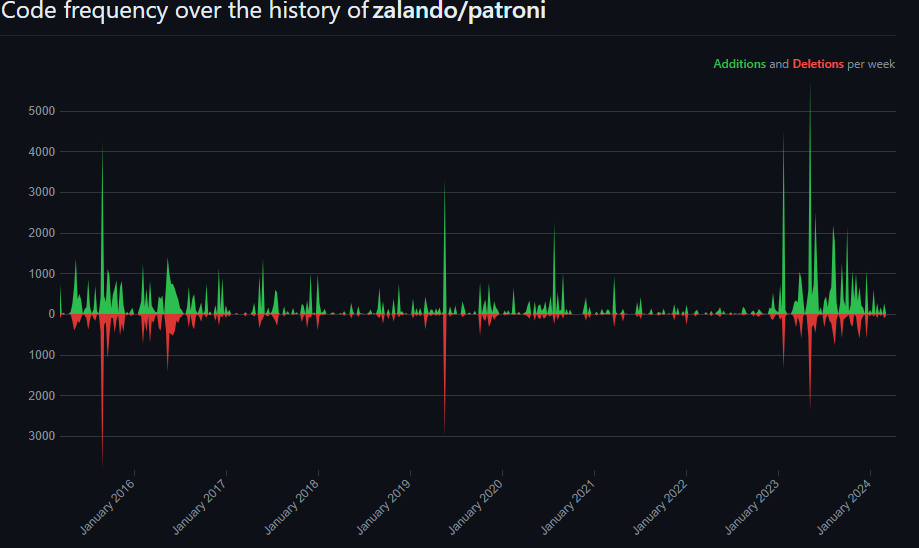
\includegraphics[width=0.75\linewidth]{source/implementation/evaluation/postgresql_ha_solutions/insights/patroni/code_frequency_zalando_patroni}
        \caption{Patroni - Code Frequency}
        \label{fig:code_frequency_zalando_patroni}
    \end{figure}
    Das Projekt hält auch die gängigen Standards auf Github ein:
    \begin{figure}[H]
        \centering
        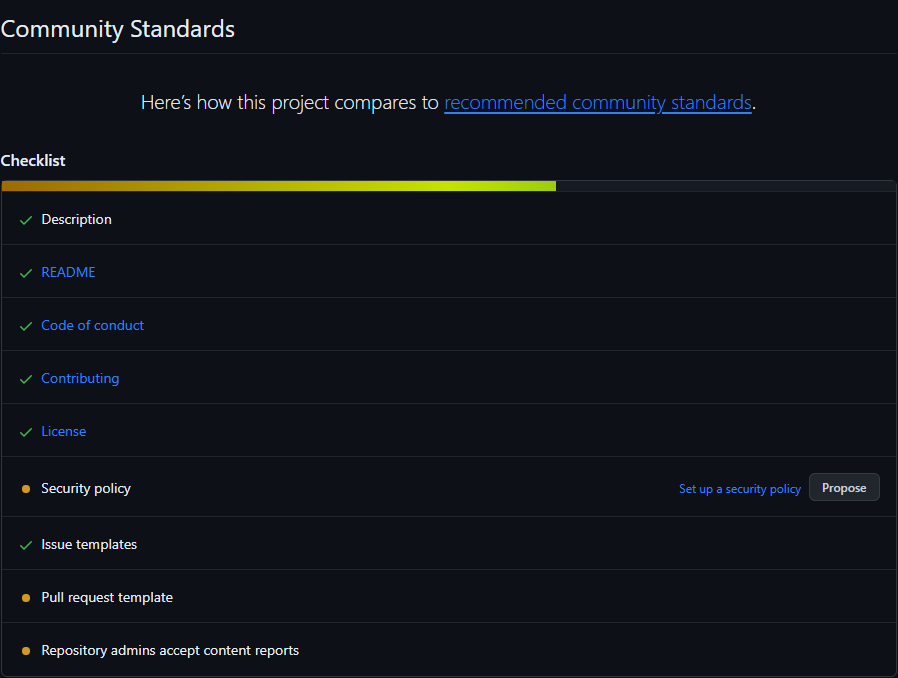
\includegraphics[width=0.75\linewidth]{source/implementation/evaluation/postgresql_ha_solutions/insights/patroni/community_Standards_zalando_patroni}
        \caption{Patroni - Community Standards}
        \label{fig:community_Standards_zalando_patroni}
    \end{figure}

    Die Contributors commiten, löschen und erweitern Patroni Regelmässig:
    \begin{figure}[H]
        \centering
        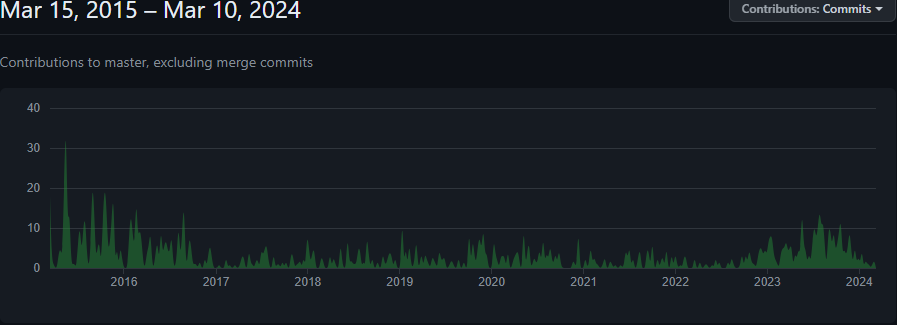
\includegraphics[width=0.75\linewidth]{source/implementation/evaluation/postgresql_ha_solutions/insights/patroni/contributors_commits_zalando_patroni}
        \caption{Patroni - Contributors Commits}
        \label{fig:contributors_commits_zalando_patroni}
    \end{figure}
    \begin{figure}[H]
        \centering
        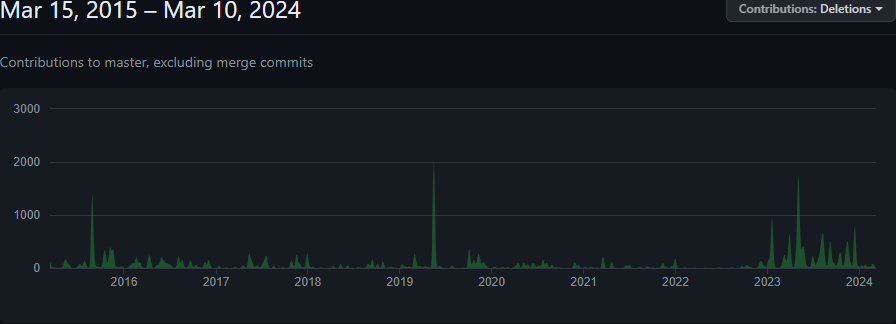
\includegraphics[width=0.75\linewidth]{source/implementation/evaluation/postgresql_ha_solutions/insights/patroni/contributors_deletations_zalando_patroni}
        \caption{Patroni - Contributors Deletations}
        \label{fig:contributors_deletations_zalando_patroni}
    \end{figure}
    \begin{figure}[H]
        \centering
        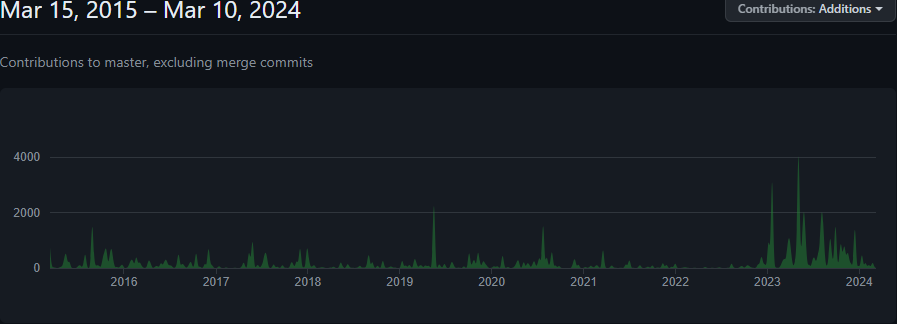
\includegraphics[width=0.75\linewidth]{source/implementation/evaluation/postgresql_ha_solutions/insights/patroni/contributors_additions_zalando_patroni}
        \caption{Patroni - Contributors Additions}
        \label{fig:contributors_additions_zalando_patroni}
    \end{figure}

    Commits werden nach wie vor immer noch Regelmässig eingespielt, auch wenn die Frequenz etwas nachgelassen hat:
    \begin{figure}[H]
        \centering
        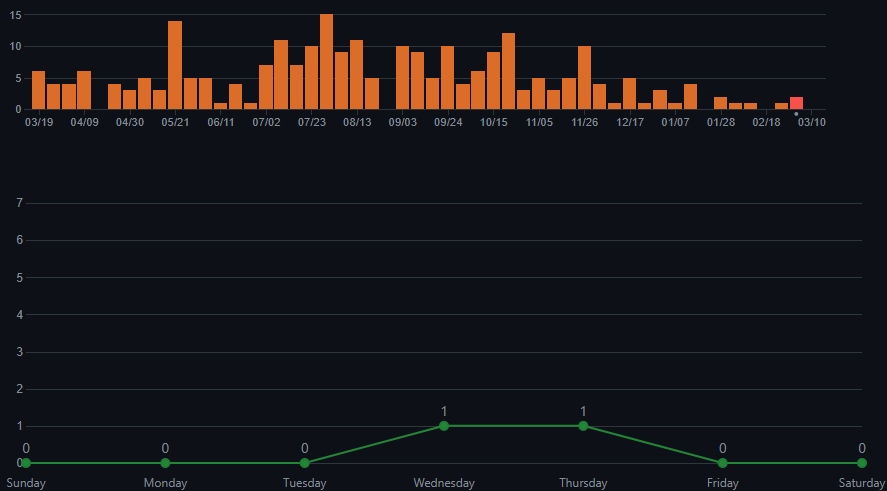
\includegraphics[width=0.75\linewidth]{source/implementation/evaluation/postgresql_ha_solutions/insights/patroni/commit_activity_zalando_patroni}
        \caption{Patroni - Commit Activity}
        \label{fig:commit_activity_zalando_patroni}
    \end{figure}

    Nebst Zalando selbst hat auch EnterpriseDB\cite{LNF967SI} ein grösseres Repository eingebunden.
    Dies weil EnterpriseDB stark auf Patroni setzt.
     \begin{figure}[H]
        \centering
        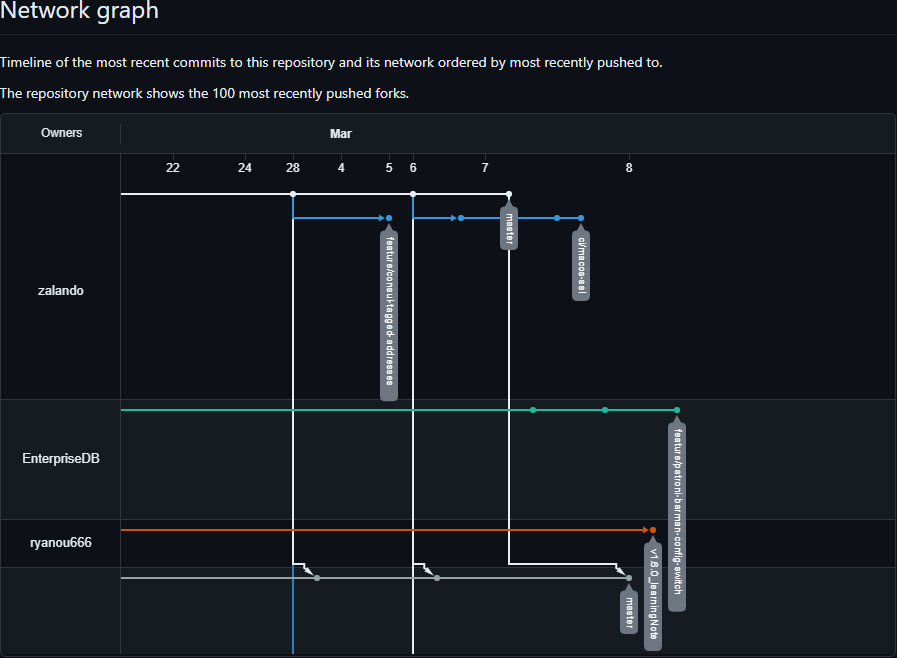
\includegraphics[width=0.75\linewidth]{source/implementation/evaluation/postgresql_ha_solutions/insights/patroni/networkgraph_zalando_patroni}
        \caption{Patroni - Network Graph}
        \label{fig:networkgraph_zalando_patroni}
    \end{figure}
\end{flushleft}